\documentclass[10pt,letterpaper]{article}
\usepackage[margin=0.8in]{geometry}
\usepackage[T1]{fontenc}
\usepackage[utf8]{inputenc}
\usepackage{lmodern}
\usepackage{amsmath,amssymb,booktabs,array,longtable}
\usepackage{pgfplots}
\pgfplotsset{compat=1.18}
\usepackage[colorlinks=true,linkcolor=blue,urlcolor=blue]{hyperref}
\usepackage{fancyhdr}
\setlength{\parindent}{0pt}
\setlength{\parskip}{5pt}
\setlength{\headheight}{14pt}
\pagestyle{fancy}\fancyhf{}
\fancyfoot[R]{\thepage}
\fancyfoot[L]{\scriptsize Research manuscript for review. Not peer reviewed. AI-assisted research and writing.}
\fancyhead[L]{\scriptsize Causal visibility repair across input orders}
\renewcommand{\headrulewidth}{0.2pt}
\definecolor{papercolor0}{HTML}{2563a6}
\definecolor{papercolor1}{HTML}{c66a24}
\definecolor{papercolor2}{HTML}{328276}
\definecolor{papercolor3}{HTML}{9961a0}
\definecolor{papercolor4}{HTML}{637082}
\definecolor{papercolor5}{HTML}{ad4747}
\title{Causal Visibility Repair Transfers Across a Finite Class of Transformer Input Orders}
\author{AI Understanding AI project}
\date{3 October 2026}
\begin{document}
\fontsize{10.5}{14.1}\selectfont
\maketitle
\begin{center}
A preregistered study of six fresh associative-recall models
\end{center}
\begin{abstract}
Changing input order changes both positional information and the sources available to causal attention. We prospectively test a fixed, structure-informed attention repair in six newly trained, two-layer transformers performing four-pair associative recall. Canonical position coordinates remain attached to token occurrences. Of 2,520 orders placing each key before its value, exactly 105 retain all native predecessors at every value position. Removing newly visible future-logical keys then restores first-layer value states algebraically, but leaves key states altered. All six models pass preregistered behavioral-recovery and mean-control comparisons across the complete 105-order class: correct-guard accuracy is 99.986-100\%, with 99.609\% the worst layout/query accuracy. The guard exceeds the within-layout mean of 624 degree-matched alternatives by 4.60-25.94 percentage points of target probability across models. On the other 2,415 orders, two stronger deletion policies achieve zero observed errors on a smaller shared input subset, although native-state restoration is not guaranteed. A separately registered single-edge redirection threshold fails in two models. These results support approximate behavioral transfer of a supplied structural repair in a finite synthetic setting, not a unique mechanism, exact answer-restoration theorem, or generalization claim for pretrained language models.
\end{abstract}
\section{Question and contribution}
Associative recall offers a controlled setting for asking whether a causal explanation predicts new behavior. A model receives four key-value pairs and must return the value associated with a query key. In earlier studies in this project, separating keys from values broke a strong position-binding account: keeping native position labels alone did not restore lookup. A subsequent fixed mask repair restored nearly all answers in those same six previously examined models [5]. The present experiment tests transfer to fresh checkpoints and an exhaustively specified family of input orders, without adjusting the repair to new shifted-layout outcomes.

The contribution is a prospective, reproducible comparison, not the discovery that context or position affects transformer behavior. We distinguish three claims: exact first-layer state identities, empirical final-answer recovery, and superiority to a specified mean control. The first follows from source-set equality; the latter two can fail. We also report a boundary panel where exact native-state recovery is not assured, and a failed secondary prediction about the magnitude of individual-edge effects.

\section{Task, models, and interventions}
Each input contains four distinct keys and four distinct values sampled independently without replacement from disjoint vocabularies of size 16. The native order is K0,V0,K1,V1,K2,V2,K3,V3,Q. Q repeats a selected key; the target is its associated value among all 16 value classes. Each model has two causal pre-LayerNorm blocks, four heads per block, residual width 64, MLP width 128, learned absolute position embeddings, and 70,720 parameters. Cross-entropy is applied only at the final query.

Seeds 6-11 and the training recipe were publicly fixed before training. Each model receives 2,000 AdamW steps at batch size 128, learning rate .001, weight decay .01, gradient clipping norm 1, and embedding initialization standard deviation 1. Every final checkpoint is retained; there is no seed replacement or performance-dependent training extension. Repeated native validation is disclosed training monitoring, not confirmation.

Canonical position IDs remain attached to their token occurrences: Ki has ID 2i, Vi has ID 2i+1, and Q has ID 8. Thus physical order changes causal visibility while preserving the input embedding of each occurrence. Q stays last. The primary correct guard removes Kj with j>i from first-layer attention at Vi, in every head, and retains other visible sources. It recomputes attention from the current layout's queries and keys with a stable masked softmax. It uses known pair identities and training coordinates, but no answers or transplanted native activations.

For each primary layout, we enumerate all key subsets of size i+1 that retain Ki at value row Vi. Their Cartesian product yields 729 masks: 105 correct guards and 624 alternatives across 102 layouts. Three layouts have no alternative. These controls match row degrees, not removed attention mass or activation-change magnitude. Unguarded, attention-reapplication no-op, and guard-plus-native-key-restoration oracle conditions bring the primary total to 1,044 layout/condition cells per model. Only the explicitly named oracle transplants native states.

The boundary panel exhausts the other 2,415 orders that place each Ki before Vi. Four fixed policies use ordinary causal visibility, delete future-logical keys, intersect visibility with the native logical prefix, or retain only Ki and Vi at each value row. We call the last policy own-key/self. The edge panel individually re-adds each of six Vi\ensuremath{\leftarrow}Kj edges with i<j to correctly guarded grouping. It tests whether Vi becomes a specific wrong competitor when the model is asked for Kj. These interventions do not constitute spontaneous discovery of the pair mapping.

\section{State restoration and its limits}
Let N(t) be the native predecessor set, including destination t, and C(t) the set available in a physical layout. With canonical coordinates, first-layer projections are unchanged. For one attention head and retained set S,

\begin{equation}
z_t(S)=\frac{\sum_{s\in S}\exp(q_t^\top k_s/\sqrt{d_h})v_s}{\sum_{s\in S}\exp(q_t^\top k_s/\sqrt{d_h})}
\end{equation}
If N(t) is contained in C(t), deleting exactly the extra sources reproduces native attention for arbitrary weights. Pointwise normalization and MLP operations preserve this equality. If a native source is missing, no deletion-only guarantee holds for arbitrary weights: uniform attention with a nonzero value only at the missing occurrence gives a counterexample. This does not imply that every trained model needs every native source.

There are 8!/2\textasciicircum{}4 = 2,520 pair-respecting orders. Every value retains all its native predecessors exactly when value order is preserved: earlier values bring their own preceding keys, whereas a reversed pair removes an earlier native value source. Pair relabeling divides the orders equally among 24 value orders, leaving 105. Their extra value predecessors are precisely future-logical keys. The guard therefore restores first-layer value states throughout this class. Q sees all tokens and has an invariant first-layer state.

First-layer key states can still differ. For a second-layer query head, let alpha be total attention mass on key positions, kappa their conditional mean projected value, and mu the shared conditional mean over value positions and Q. Subscripts g and n denote guarded and native computation:

\begin{equation}
z_g-z_n=\alpha_g(\kappa_g-\mu)-\alpha_n(\kappa_n-\mu)
\end{equation}
Changes to both key content and attention normalization remain possible. Later nonlinearities can turn them into output errors. Final-answer recovery is therefore an empirical question. Separately, own-key/self makes first-layer value states invariant under every pair-respecting layout, but generally does not make them native. These elementary identities define manipulation checks and scope; they are not claimed as new general theorems. The full proof and missing-source construction are preserved with the registration [5].

\section{Prospective protocol and analysis}
Primary and edge panels use 1,024 fresh dictionaries, balanced at 256 per query position. The boundary panel uses the first 256 accepted dictionaries, balanced at 64 per position; it is not an independent dataset. Input selection is independent of outputs. Rejection checks all 96 native pair-order/query variants against historical inputs and all six new training streams. A further exclusion of earlier grouped token bags covers alternative pairings. An independent generation audit checked 10,321,920 legal layout/query representations against 4,393,029 prior exact identities, with no overlap.

Registration de745644b5c71853755e8d53cc9b3dec2abdc2ed freezes code, inputs, checkpoints, conditions, gates, and forecasts. All 96 file identities were remotely verified at 16:46:17 UTC on 3 October 2026; confirmatory evaluation began at 16:46:45 UTC. E1-E4 remain disclosed discovery history, including E3's failed strong claim. Implementation, blinded prediction, and skeptical review used separate AI-agent roles. Their shared-filesystem separation was procedural, not a security boundary or independent human replication.

Validity requires native accuracy at least .95; complete, finite, normalized, consistent saved class outputs; no-op discrepancies at most 1e-6; and registered state/oracle discrepancies at most 1e-5. Every fresh model must then pass three primary criteria: accuracy at least .95 in every one of 105\ensuremath{\times}4 layout/query cells; a paired 95\% upper bound at most .01 on mean native-minus-guard target probability; and a paired 95\% lower bound greater than .02 on guard-minus-mean-alternatives probability. The native comparison is signed noninferiority, not an absolute-discrepancy bound. Controls are averaged within layout, then equally across 102 eligible layouts.

Intervals use 2,000 paired dictionary-row bootstrap samples within query strata, with shared weights across conditions, layouts, and models. Layout aggregation precedes resampling. These intervals condition on the six checkpoints; they do not estimate uncertainty over the population of possible training runs. The 21,301,248 saved case-condition rows are repeated interventions, not independent replications. Per-cell Wilson intervals are pointwise, not simultaneous confidence bands.

Separate all-model secondary gates require pooled boundary accuracy at least .95 for logical-prefix and own-key/self policies, and an edge-enrichment lower bound greater than .05. The edge endpoint subtracts the mean change for the other two displayed wrong values from the change in P(Vi), relative to the guarded base. Only queries for the re-added source Kj contribute; the six edge means receive equal weight. Separately, a blinded agent fixed 72 aggregate numerical forecasts with absolute tolerance .05. Forecast scores and secondary success cannot replace a failed primary criterion.

\section{Results}
All six models pass every validity and primary criterion. Native accuracy is 100\%. Unguarded accuracy over the same primary layouts is 45.2-71.9\% across models. Five models make no correct-guard primary errors; seed 7 makes 15 errors among 107,520 layout/case combinations, for 99.9860\% accuracy. Those errors involve two dictionaries across 15 layouts. The worst layout/query cell is 255/256 correct (99.6094\%). No primary cell fails its .95 threshold. These results establish approximate, not exact, recovery.

\begin{longtable}{@{}>{\raggedright\arraybackslash}p{\dimexpr 0.16667\linewidth-2\tabcolsep\relax}>{\raggedright\arraybackslash}p{\dimexpr 0.16667\linewidth-2\tabcolsep\relax}>{\raggedright\arraybackslash}p{\dimexpr 0.16667\linewidth-2\tabcolsep\relax}>{\raggedright\arraybackslash}p{\dimexpr 0.16667\linewidth-2\tabcolsep\relax}>{\raggedright\arraybackslash}p{\dimexpr 0.16667\linewidth-2\tabcolsep\relax}>{\raggedright\arraybackslash}p{\dimexpr 0.16667\linewidth-2\tabcolsep\relax}@{}}
\caption{Complete fresh cohort. Loss upper is the paired 95\% upper bound on native-minus-guard target probability; control gain is guard minus the mean alternatives. All probability differences are percentage points (pp). Native accuracy is 100\% for every seed.}\\
\toprule
\textbf{Seed} & \textbf{Guard acc. (\%)} & \textbf{Worst cell (\%)} & \textbf{Loss upper (pp)} & \textbf{Control gain (pp)} & \textbf{Primary}\\
\midrule\endhead
6 & 100.0000 & 100.00 & 0.0004 & 9.80 & Pass\\
7 & 99.9860 & 99.61 & 0.0623 & 20.64 & Pass\\
8 & 100.0000 & 100.00 & 0.0013 & 11.75 & Pass\\
9 & 100.0000 & 100.00 & 0.0027 & 25.94 & Pass\\
10 & 100.0000 & 100.00 & 0.0004 & 4.60 & Pass\\
11 & 100.0000 & 100.00 & 0.0054 & 15.02 & Pass\\
\bottomrule
\end{longtable}
\begin{figure}[htbp]
\centering
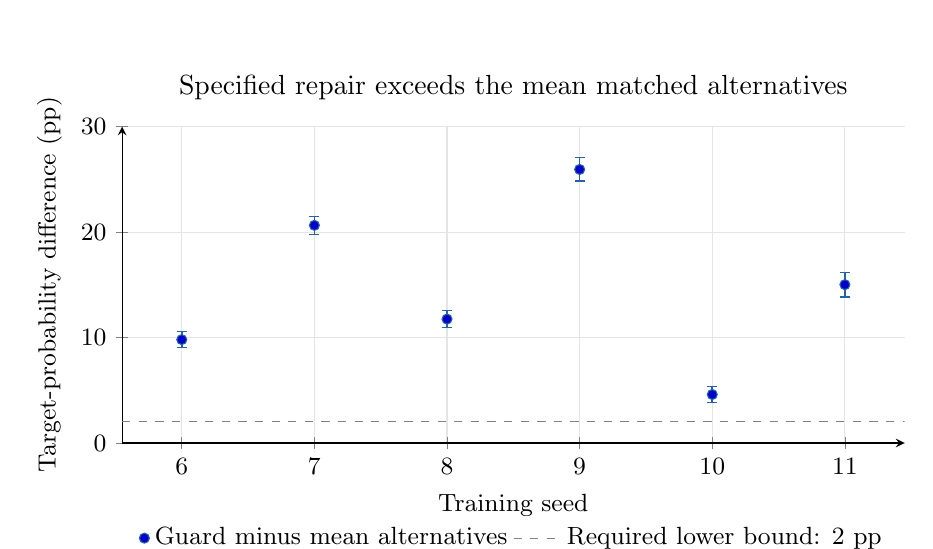
\begin{tikzpicture}
\begin{axis}[width=0.95\linewidth,
height=5.6cm,
grid=major,
major grid style={gray!20},
axis lines=left,
tick label style={font=\small},
label style={font=\small},
xtick={0,1,2,3,4,5},
xticklabels={{6},{7},{8},{9},{10},{11}},
ylabel={Target-probability difference (pp)},
title={Specified repair exceeds the mean matched alternatives},
xlabel={Training seed},
legend style={at={(0.5,-0.23)},anchor=north,draw=none,font=\small},
legend columns=2,
ymin=0,
ymax=30]
\addplot+[color=papercolor0,fill=papercolor0,only marks,mark=*,mark size=1.8pt,error bars/.cd,y dir=both,y explicit,error bar style={line width=.6pt}] coordinates {
(0.0,9.803751984376891) += (0,0.7895424616925393) -= (0,0.7480704041057713)
(1.0,20.64110819376653) += (0,0.8352258897098785) -= (0,0.8620327404945662)
(2.0,11.7523043308146) += (0,0.8332695954804272) -= (0,0.8204235707464882)
(3.0,25.93844652297022) += (0,1.1173853559997333) -= (0,1.0936501551380253)
(4.0,4.600987971381867) += (0,0.7712256144929714) -= (0,0.7298176344553382)
(5.0,15.016433540206778) += (0,1.16504678305518) -= (0,1.1747194779760477)
};
\addlegendentry{Guard minus mean alternatives}
\addplot[gray,dashed,domain=-0.45:5.45,samples=2] {2};
\addlegendentry{Required lower bound: 2 pp}
\end{axis}
\end{tikzpicture}
\caption{Points and paired 95\% intervals for all six seeds. Every lower bound exceeds the registered 2-point requirement. Within-layout averaging prevents layouts with more alternatives from receiving greater weight. This comparison does not establish superiority to each alternative.}
\label{fig:control_gain}
\end{figure}
Mean-control gains range from 4.60 to 25.94 percentage points. All lower confidence bounds exceed 2 points. The largest upper bound for native-minus-guard probability is .000624, below the .01 limit. No-op outputs are identical. Maximum correct-guard value-state error is 1.91e-6; maximum full-oracle probability error is 2.38e-7. These last quantities validate implementation of identities, rather than add independent evidence for behavioral recovery. One seed-7 failure reduces target probability from .999083 to .008674 despite restored value states. The oracle restores native output probabilities for these failures as well.

\begin{figure}[htbp]
\centering
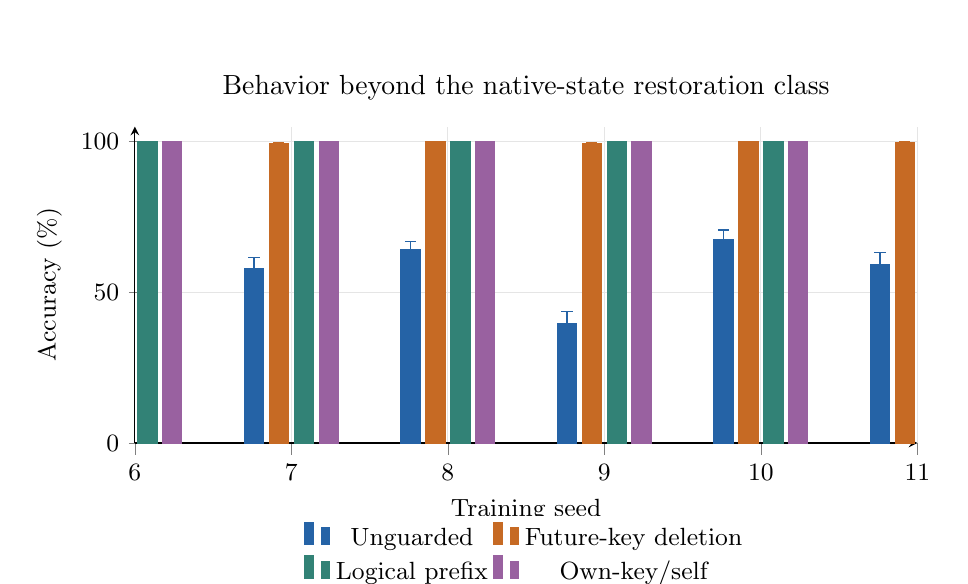
\begin{tikzpicture}
\begin{axis}[width=0.95\linewidth,
height=5.6cm,
grid=major,
major grid style={gray!20},
axis lines=left,
tick label style={font=\small},
label style={font=\small},
xtick={0,1,2,3,4,5},
xticklabels={{6},{7},{8},{9},{10},{11}},
ylabel={Accuracy (\%)},
title={Behavior beyond the native-state restoration class},
xlabel={Training seed},
legend style={at={(0.5,-0.23)},anchor=north,draw=none,font=\small},
legend columns=2,
ymin=0,
ymax=105,
ybar,
bar width=7pt]
\addplot+[color=papercolor0,fill=papercolor0,error bars/.cd,y dir=both,y explicit,error bar style={line width=.6pt}] coordinates {
(0,68.57676630434783) += (0,3.5817037072981464) -= (0,3.5182776915113863)
(1,58.062241200828154) += (0,3.6042515851449295) -= (0,3.5955494629917197)
(2,64.06945522774326) += (0,2.884535131987576) -= (0,2.942732595755679)
(3,39.568614130434774) += (0,3.9986696105072568) -= (0,3.824631211180119)
(4,67.51714544513457) += (0,3.187803280279482) -= (0,3.178284323240163)
(5,59.26840709109731) += (0,3.830231787008273) -= (0,3.9672902109213126)
};
\addlegendentry{Unguarded}
\addplot+[color=papercolor1,fill=papercolor1,error bars/.cd,y dir=both,y explicit,error bar style={line width=.6pt}] coordinates {
(0,99.6591938405797) += (0,0.3291601966873827) -= (0,0.446537752329192)
(1,99.26501035196688) += (0,0.5619257893374652) -= (0,0.7186003817287911)
(2,100.0) += (0,0.0) -= (0,0.0)
(3,99.48385740165632) += (0,0.38787930253621994) -= (0,0.5038739001035282)
(4,100.0) += (0,0.0) -= (0,0.0)
(5,99.7547877846791) += (0,0.24521221532090465) -= (0,0.3969332298136692)
};
\addlegendentry{Future-key deletion}
\addplot+[color=papercolor2,fill=papercolor2,error bars/.cd,y dir=both,y explicit,error bar style={line width=.6pt}] coordinates {
(0,100.0) += (0,0.0) -= (0,0.0)
(1,100.0) += (0,0.0) -= (0,0.0)
(2,100.0) += (0,0.0) -= (0,0.0)
(3,100.0) += (0,0.0) -= (0,0.0)
(4,100.0) += (0,0.0) -= (0,0.0)
(5,100.0) += (0,0.0) -= (0,0.0)
};
\addlegendentry{Logical prefix}
\addplot+[color=papercolor3,fill=papercolor3,error bars/.cd,y dir=both,y explicit,error bar style={line width=.6pt}] coordinates {
(0,100.0) += (0,0.0) -= (0,0.0)
(1,100.0) += (0,0.0) -= (0,0.0)
(2,100.0) += (0,0.0) -= (0,0.0)
(3,100.0) += (0,0.0) -= (0,0.0)
(4,100.0) += (0,0.0) -= (0,0.0)
(5,100.0) += (0,0.0) -= (0,0.0)
};
\addlegendentry{Own-key/self}
\end{axis}
\end{tikzpicture}
\caption{All 2,415 boundary orders on the shared 256-dictionary subset. Bars show equal-layout mean accuracy with paired 95\% intervals. Logical-prefix and own-key/self have zero observed errors in every model; their empirical bootstrap intervals are degenerate and do not imply zero population risk.}
\label{fig:boundary_policies}
\end{figure}
Unguarded boundary accuracy ranges from 39.57\% to 68.58\%. Deleting future keys alone raises it to 99.27-100\%. Logical-prefix and own-key/self both achieve 100\% on every tested boundary case. Under these two policies, all individual boundary layout/query cells also meet .95, though that fraction is descriptive. The fixed-key-order subset has the same qualitative pattern. Its 23 boundary value orders and the primary grouped reference are reported separately in the full results, avoiding an average over missing policies or mixed samples.

The boundary result separates behavioral sufficiency from exact native-state recovery. Missing native sources can defeat a universal restoration guarantee without preventing the trained models from answering. It does not establish the smallest sufficient circuit or show that the model can infer our externally supplied mask.

\begin{figure}[htbp]
\centering
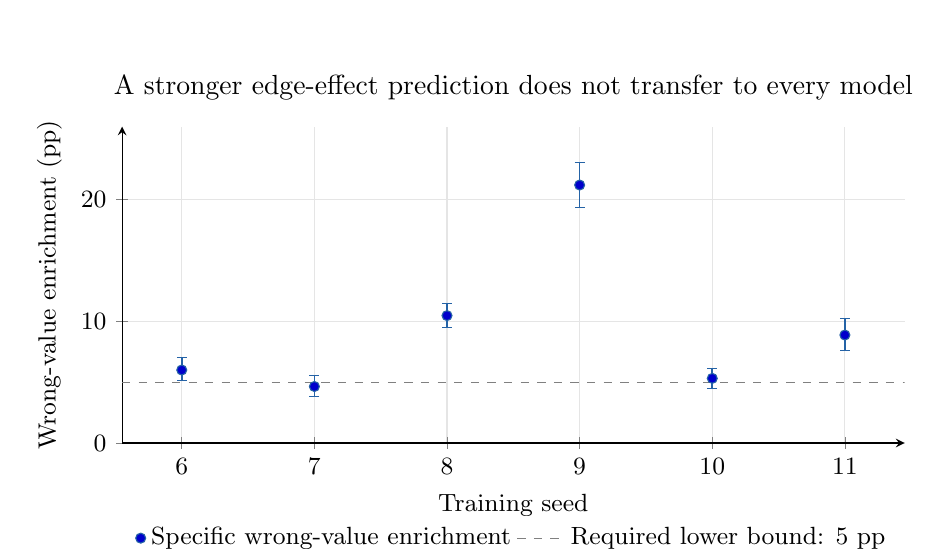
\begin{tikzpicture}
\begin{axis}[width=0.95\linewidth,
height=5.6cm,
grid=major,
major grid style={gray!20},
axis lines=left,
tick label style={font=\small},
label style={font=\small},
xtick={0,1,2,3,4,5},
xticklabels={{6},{7},{8},{9},{10},{11}},
ylabel={Wrong-value enrichment (pp)},
title={A stronger edge-effect prediction does not transfer to every model},
xlabel={Training seed},
legend style={at={(0.5,-0.23)},anchor=north,draw=none,font=\small},
legend columns=2,
ymin=0,
ymax=26]
\addplot+[color=papercolor0,fill=papercolor0,only marks,mark=*,mark size=1.8pt,error bars/.cd,y dir=both,y explicit,error bar style={line width=.6pt}] coordinates {
(0.0,6.000217708790688) += (0,1.0000220813673169) -= (0,0.8762912737798514)
(1.0,4.6453703233000905) += (0,0.8933858690548009) -= (0,0.8328019140311591)
(2.0,10.470842428227584) += (0,0.9921194998355478) -= (0,0.9601406584250718)
(3.0,21.1996413087889) += (0,1.8248230019882037) -= (0,1.8552182197427278)
(4.0,5.312677221277768) += (0,0.8217900256775055) -= (0,0.8121909479115743)
(5.0,8.875625840631878) += (0,1.3628312795180424) -= (0,1.2753064513892793)
};
\addlegendentry{Specific wrong-value enrichment}
\addplot[gray,dashed,domain=-0.45:5.45,samples=2] {5};
\addlegendentry{Required lower bound: 5 pp}
\end{axis}
\end{tikzpicture}
\caption{Equal-edge enrichment and paired 95\% intervals. Seeds 7 and 10 fail the registered lower-bound threshold; the all-six secondary claim fails. Positive direction alone does not satisfy the stronger preregistered prediction.}
\label{fig:edge_enrichment}
\end{figure}
The edge endpoint is positive in all six models, but its required lower bound exceeds .05 only in seeds 6, 8, 9, and 11. Seeds 7 and 10 have lower bounds .0381 and .0450. We retain this failed secondary claim without changing its threshold. Of the 72 aggregate point forecasts, 65 fall within .05; mean absolute error is 0.0208 and RMSE is 0.0360. Every miss and every wrong primary prediction is retained [5].

\section{Relation to prior work}
Arora et al. [1] use causal interventions to analyze association and retrieval, including information carried at value positions, across transformer and state-space architectures. That is close precedent for the binding mechanisms studied here. Our narrower addition is a frozen repair tested prospectively across a complete finite serialization class and fresh seeds, with full matched-mask enumeration.

Wu et al. [2] analyze attention masks as directed graphs and their interaction with positional encodings. Causal visibility is therefore an established explanatory variable. Tang, Lake, and Jazayeri [3] identify positional and token-information pathways and demonstrate partial steering through positional interventions. We claim neither the first position-based explanation nor the first causal manipulation of associative recall.

Geng et al. [4] show that intervention-based faithfulness objectives can misrank candidate circuits and study partial computational-context restoration. Their ranking endpoint differs from our answer-recovery endpoint, but the conceptual overlap is substantial. Our controls, native-state oracle, and behavioral gates address different questions; their agreement still cannot identify a unique internal algorithm. These sources were checked on 3 October 2026; no field-wide priority claim is made.

\section{Limits, next tests, and reproducibility}
The evidence is conditional on one tiny two-layer architecture, four pairs, learned absolute coordinates, and six fixed training seeds. Canonical IDs retain training-slot information, and masks use known pair identities. This is not ordinary position-invariant generalization. Complete layout coverage does not remove uncertainty over unseen dictionaries, architectures, longer sequences, or training runs. Count-matched controls also leave attention-mass and activation-norm confounds for finer mechanistic interpretations.

The most useful next tests are external replication, longer lists and deeper models, controls matched for attention mass, and policies that infer pair structure instead of receiving it. A separate preregistration should specify each expanded claim before new outcomes. The boundary success suggests studying how little context is behaviorally sufficient; it does not itself establish minimality. Applying the intervention to pretrained language models requires new evidence.

All experimental training and inference used a local Apple M3 MacBook Air with 16 GiB RAM and four CPU threads. The six in-process training timers total approximately 94.44 seconds, excluding process startup. Confirmatory evaluation took 23.43 minutes from start to finish, excluding scoring and earlier studies. The 492 raw shards occupy 2.025 GB in decimal units. Python 3.14.8, PyTorch 2.14.1, and NumPy 2.5.3 are pinned; no inference API was used for the model experiments. Conversational AI research roles were provided by Codex, not local model inference.

The public repository contains immutable registration history, all checkpoints, full saved class probabilities, completion hashes, all conditions and failures, and a reproduction guide [5]. The scorer performs no model forwards. A separate audit recomputes aggregates and decisions from raw shards; saved state discrepancies remain runner measurements supported by synthetic implementation tests. Separate AI-agent review is an internal audit, not external peer review. The manuscript and figures are generated from a shared JSON record by paper/assemble.py and paper/build.py. Research, code, analysis, and writing used AI assistance; human authorship and any venue submission require the responsible researchers' review.

\begin{thebibliography}{99}
\bibitem[1]{1} Arora A, Rathi N, Selvam NR, Csordás R, Jurafsky D, Potts C. Mechanistic evaluation of Transformers and state space models. arXiv:2505.15105, v3, 30 January 2026 (original 2025).
\url{https://arxiv.org/abs/2505.15105}.
\bibitem[2]{2} Wu X, Wang Y, Jegelka S, Jadbabaie A. On the Emergence of Position Bias in Transformers. ICML 2025; arXiv:2502.01951, v4, 9 August 2025.
\url{https://arxiv.org/abs/2502.01951}.
\bibitem[3]{3} Tang C, Lake B, Jazayeri M. Circuit explained: How does a transformer perform compositional generalization. PLOS ONE, 4 February 2026, e0340088.
\url{https://journals.plos.org/plosone/article?id=10.1371/journal.pone.0340088}.
\bibitem[4]{4} Geng C, Zhang L, Ye H, Zhang M, Zhang L, Si X. Are We Recovering Mechanisms? Objective-Level Recovery Gaps in Mechanistic Interpretability. arXiv:2610.02098, v1, 1 October 2026. Preprint.
\url{https://arxiv.org/abs/2610.02098}.
\bibitem[5]{5} AI Understanding AI project. Experiment 5 protocol, theory, frozen registration, results, audits, and reproduction package. 3 October 2026. Registration: de745644b5c71853755e8d53cc9b3dec2abdc2ed.
\url{https://github.com/posix4e/ai-understanding-ai}.
\end{thebibliography}
\end{document}
